	\chapter[DeepPoseKit]{DeepPoseKit: a software toolkit for fast and robust animal pose estimation using deep learning \blfootnote{\textbf{Adapted from:} Graving, J. M., Chae, D., Naik, H., Li, L., Koger, B., Costelloe, B. R., & Couzin, I. D. (2019). DeepPoseKit, a software toolkit for fast and robust animal pose estimation using deep learning. eLife, 8, e47994 under a CC-BY-4.0 International License  \ccby} \\ \vspace{10mm} \Large Jacob M. Graving, Daniel Chae, Hemal Naik, Liang Li, Benjamin Koger, Blair R. Costelloe, and Iain D. Couzin}
	\normalsize
\newpage
\section{Abstract}
    Quantitative behavioral measurements are important for answering questions across scientific disciplines---from neuroscience to ecology. State-of-the-art deep-learning methods offer major advances in data quality and detail by allowing researchers to automatically estimate locations of an animal's body parts directly from images or videos. However, currently-available animal pose estimation methods have limitations in speed and robustness. Here we introduce a new easy-to-use software toolkit, \textit{DeepPoseKit}, that addresses these problems using an efficient multi-scale deep-learning model, called \textit{Stacked DenseNet}, and a fast GPU-based peak-detection algorithm for estimating keypoint locations with subpixel precision. These advances improve processing speed $>$2$\times$ with no loss in accuracy compared to currently-available methods. We demonstrate the versatility of our methods with multiple challenging animal pose estimation tasks in laboratory and field settings---including groups of interacting individuals. Our work reduces barriers to using advanced tools for measuring behavior and has broad applicability across the behavioral sciences.



\section{Introduction}
Understanding the relationships between individual behavior, brain activity (reviewed by \citealt{krakauer2017neuroscience}), and collective and social behaviors \citep{rosenthal2015revealing,strandburg2013visual, jolles2017consistent, klibaite2017unsupervised, klibaite2019interacting} is a central goal of the behavioral sciences—a field that spans disciplines from neuroscience to psychology, ecology, and genetics. Measuring and modeling behavior is key to understanding these multiple scales of complexity, and, with this goal in mind, researchers in the behavioral sciences have begun to integrate theory and methods from physics, computer science, and mathematics \citep{anderson2014toward, berman2018measuring, brown2018ethology}. A cornerstone of this interdisciplinary revolution is the use of state-of-the-art computational tools, such as computer vision algorithms, to automatically measure locomotion and body posture \citep{dell2014automated}. Such a rich description of animal movement then allows for modeling, from first principles, the full behavioral repertoire of animals \citep{stephens2011emergence, berman2014mapping, berman2016predictability, wiltschko2015mapping, johnson2016composing, todd2017systematic, klibaite2017unsupervised, markowitz2018striatum, klibaite2019interacting,Costa1501}. Tools for automatically measuring animal movement represent a vital first step toward developing unified theories of behavior across scales \citep{berman2018measuring, brown2018ethology}. Therefore, technical factors like scalability, robustness, and usability are issues of critical importance, especially as researchers across disciplines begin to increasingly rely on these methods.


Two of the latest contributions to the growing toolbox for quantitative behavioral analysis are from \cite{mathis2018deeplabcut} and \cite{pereira2019fast}, who make use of a popular type of machine learning model called \textit{convolutional neural networks}, or \textit{CNNs} (\citealt{lecun2015deep}; Appendix \ref{app:cnn}), to automatically measure detailed representations of animal posture—structural \textit{keypoints}, or \textit{joints}, on the animal's body—directly from images and without markers. While these methods offer a major advance over conventional methods with regard to data quality and detail, they have disadvantages in terms of speed and robustness, which may limit their practical applications. 
To address these problems, we introduce a new software toolkit, called \textit{DeepPoseKit}, with methods that are fast, robust, and easy-to-use. We run experiments using multiple datasets to compare our new methods with those from \cite{mathis2018deeplabcut} and \cite{pereira2019fast}, and we find that our approach offers considerable improvements. These results also demonstrate the flexibility of our toolkit for both laboratory and field situations and exemplify the wide applicability of our methods across a range of species and experimental conditions.

\begin{figure}[!htb]
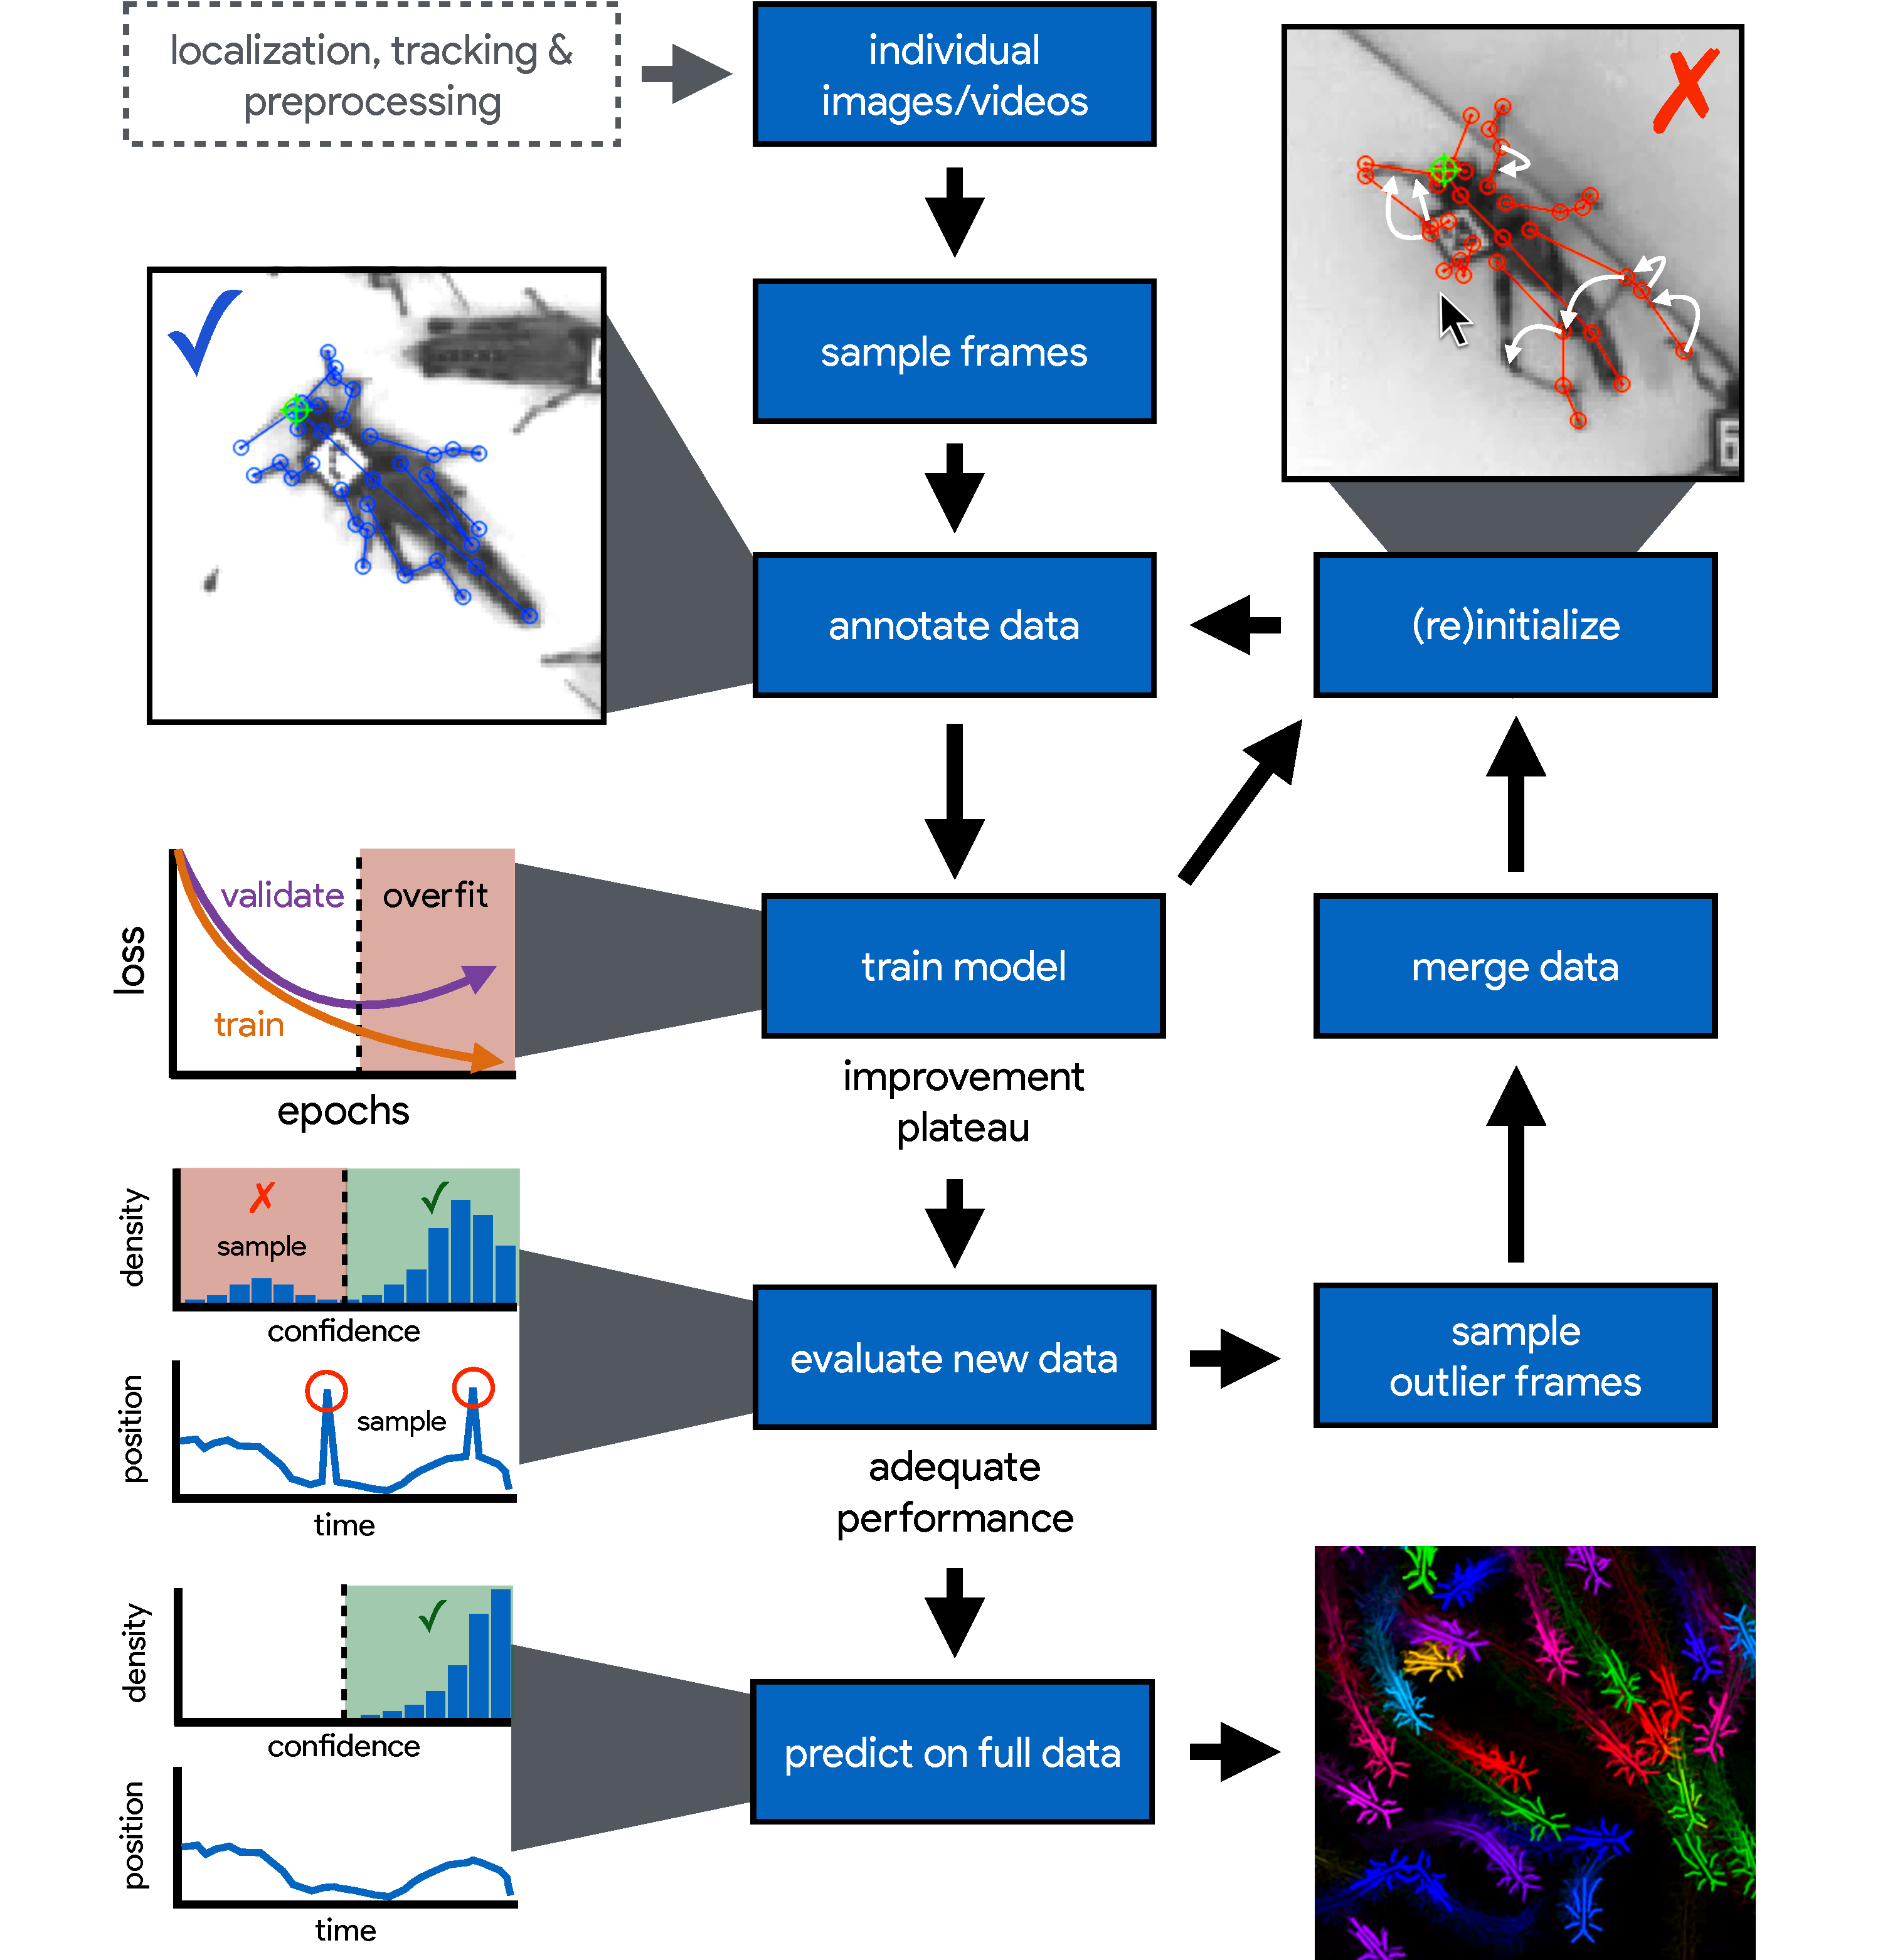
\includegraphics[width=0.95\linewidth]{Graving_IMPRS_Thesis/figures/workflow_figure.pdf}

\caption{An illustration of the workflow for DeepPoseKit. Multi-individual images are localized, tracked, and preprocessed into individual images, which is not required for single-individual image datasets. An initial image set is sampled, annotated, and then iteratively updated using the active learning approach described by \cite{pereira2019fast} (see Appendix \ref{app:training_data}). As annotations are made, the model is trained (Figure \ref{fig:model_training_figure}) with the current training set and keypoint locations are initialized for unannotated data to reduce the difficulty of further annotations. This is repeated until there is a noticeable improvement plateau for the initialized data---where the annotator is providing only minor corrections---and for the validation error when training the model (Appendix \ref{app:figures} Figure \ref{fig:training_prop}). New data from the full dataset are evaluated with the model, and the training set is merged with new examples that are sampled based on the model's predictive performance, which can be assessed with techniques described by \cite{mathis2018deeplabcut, nath2018} for identifying outlier frames and minimizing extreme prediction errors—shown here as the distribution of confidence scores predicted by the model and predicted body part positions with large temporal derivatives---indicating extreme errors. This process is repeated as necessary until performance is adequate when evaluating new data. The pose estimation model can then be used to make predictions for the full data set, and the data can be used for further analysis.}
\label{fig:workflow_figure}
\end{figure}

\begin{figure}[!htb]
    \centering
    \includegraphics{}
    \caption{A visualization of the posture data output for a group of locusts (5$\times$ speed) \url{https://youtu.be/hCa2zaoUWhs}
}
\end{figure}

\subsection{Measuring animal movement with computer vision}
Collecting high-quality behavioral data is a challenging task, and while direct observations are important for gathering qualitative data about a study system, a variety of automated methods for quantifying movement have become popular in recent years \citep{dell2014automated, anderson2014toward, kays2015terrestrial}. Methods like video monitoring and recording help to accelerate data collection and reduce the effects of human intervention, but the task of manually scoring videos is time consuming and suffers from the same limitations as direct observation, namely observer bias and mental fatigue. Additionally, due to limitations of human observers' ability to process information, many studies that rely on manual scoring use relatively small datasets to estimate experimental effects, which can lead to increased rates of statistical errors. Studies that lack the statistical resolution to robustly test hypotheses (commonly called "power" in frequentist statistics) also raise concerns about the use of animals for research, as statistical errors caused by sparse data can impact researchers' ability to accurately answer scientific questions. These limitations have led to the development of automated methods for quantifying behavior using advanced imaging technologies \citep{dell2014automated} as well as sophisticated tags and collars with GPS, accelerometry, and acoustic-recording capabilities \citep{kays2015terrestrial}. Tools for automatically measuring the behavior of individuals now play a central role in our ability to study the neurobiology and ecology of animals, and reliance on these technologies for studying animal behavior will only increase in the future.

The rapid development of computer vision hardware and software in recent years has allowed for the use of automated image-based methods for measuring behavior across many experimental contexts \citep{dell2014automated}. Early methods for quantifying movement with these techniques required highly-controlled laboratory conditions. However, because animals exhibit different behaviors depending on their surroundings \citep{strandburg2017habitat,francisco2020high, akhund2019effect}, laboratory environments are often less than ideal for studying many natural behaviors. Most conventional computer vision methods are also limited in their ability to accurately track groups of individuals over time, but nearly all animals are social at some point in their life and exhibit specialized behaviors when in the presence of conspecifics \citep{strandburg2013visual, rosenthal2015revealing, jolles2017consistent,klibaite2017unsupervised,klibaite2019interacting, francisco2020high, versace2019individual}. These methods also commonly track only the animal's center of mass, which reduces the behavioral output of an individual to a two-dimensional or three-dimensional particle-like trajectory. While trajectory data are useful for many experimental designs, the behavioral repertoire of an animal cannot be fully described by its aggregate locomotory output. For example, stationary behaviors, like grooming and antennae movements, or subtle differences in walking gaits cannot be reliably detected by simply tracking an animal's center of mass \citep{berman2014mapping, wiltschko2015mapping}. 

Together these factors have driven the development of software that can accurately track the positions of marked \citep{crall2015beetag, graving2017pinpoint, wild2018honeybee, boenisch2018tracking} or unmarked \citep{perez2014idtracker, romero2018idtracker} individuals as well as methods that can quantify detailed descriptions of an animal's posture over time \citep{stephens2011emergence, berman2014mapping, wiltschko2015mapping, mathis2018deeplabcut, pereira2019fast}. Recently these advancements have been further improved through the use of deep learning, a class of machine learning algorithms that learn complex statistical relationships from data \citep{lecun2015deep}. Deep learning has opened the door to accurately tracking large groups of marked \citep{wild2018honeybee, boenisch2018tracking} or unmarked \citep{romero2018idtracker} individuals and has made it possible to measure the body posture of animals in nearly any context---including in the wild \citep{nath2018}---by tracking the positions of user-defined body parts \citep{mathis2018deeplabcut, pereira2019fast}. These advances have drastically increased the quality and quantity, as well as the diversity, of behavioral data that are potentially available to researchers for answering scientific questions.

\subsection{Animal pose estimation using deep learning}
In the past, conventional methods for measuring posture with computer vision relied on species-specific algorithms \citep{uhlmann2017flylimbtracker}, highly-specialized or restrictive experimental setups \citep{mendes2013quantification, kain2013leg}, attaching intrusive physical markers to the study animal \citep{kain2013leg}, or some combination thereof. These methods also typically required expert computer-vision knowledge to use, were limited in the number or type of body parts that could be tracked \citep{mendes2013quantification}, involved capturing and handling the study animals to attach markers \citep{kain2013leg}---which is not possible for many species---and despite best efforts to minimize human involvement, often required manual intervention to correct errors \citep{uhlmann2017flylimbtracker}. All of these methods were built to work for a small range of conditions and typically required considerable effort to adapt to novel contexts.

In contrast to conventional computer-vision methods, modern deep-learning–based methods can be used to achieve near human-level accuracy in almost any scenario by manually annotating data (Figure \ref{fig:workflow_figure})—known as a \textit{training set}—and training a general-purpose image-processing algorithm—a convolutional neural network or CNN—to automatically estimate the locations of an animal's body parts directly from images (Figure \ref{fig:model_training_figure}). State-of-the-art machine learning methods, like CNNs, use these training data to parameterize a model describing the statistical relationships between a set of input data—i.e., images—and the desired output distribution—i.e., posture keypoints. After adequate training, a model can be used to make predictions on previously-unseen data from the same dataset—inputs that were not part of the training set, which is known as \textit{inference}. In other words, these models are able to generalize human-level expertise at scale after having been trained on only a relatively small number of examples. We provide more detailed background information on using CNNs for pose estimation in Appendices \ref{app:cnn}–\ref{app:overparam}.

Similar to conventional pose estimation methods, the task of implementing deep-learning models in software and training them on new data is complex and requires expert knowledge. However, in most cases, once the underlying model and training routine are implemented, a high-accuracy pose estimation model for a novel context can be built with minimal modification—often just by changing the training data. With a simplified toolkit and high-level software interface designed by an expert, even scientists with limited computer-vision knowledge can begin to apply these methods to their research. Once the barriers for implementing and training a model are sufficiently reduced, the main bottleneck for using these methods becomes collecting an adequate training set—a labor-intensive task made less time-consuming by techniques described in Appendix \ref{app:training_data}.

\cite{mathis2018deeplabcut} and \cite{pereira2019fast} were the first to popularize the use of CNNs for animal pose estimation. These researchers built on work from the human pose estimation literature (e.g., \citealt{andriluka14cvpr,insafutdinov2016deepercut,newell2016}) using a type of \textit{fully-convolutional neural network} or \textit{F-CNN} (\citealt{long2015fully}; Appendix \ref{app:fcnn}) often referred to as an \textit{encoder-decoder} model (Appendix \ref{app:fcnn} Box \ref{box:encoder_decoder_box}). These models are used to measure animal posture by training the network to transform images into probabilistic estimates of keypoint locations, known as \textit{confidence maps} (shown in Figure \ref{fig:model_training_figure}), that describe the body posture for one or more individuals. These confidence maps are processed to produce the 2-D spatial coordinates of each keypoint, which can then be used for further analysis. 

While deep-learning models typically need large amounts of training data, both \cite{mathis2018deeplabcut} and \cite{pereira2019fast} have demonstrated that near human-level accuracy can be achieved with few training examples (Appendix \ref{app:training_data}). In order to ensure generalization to large datasets, both groups of researchers introduced ideas related to iteratively refining the training set used for model fitting \citep{mathis2018deeplabcut, pereira2019fast}. In particular, \cite{pereira2019fast} describe a technique known as \textit{active learning} where a trained model is used to initialize new training data and reduce annotation time (Appendix \ref{app:training_data}). \cite{mathis2018deeplabcut} describe multiple techniques that can be used to further refine training data and minimize errors when making predictions on the full dataset. Simple methods to accomplish this include filtering data or selecting new training examples based on confidence scores or the entropy of the confidence maps from the model output. \cite{nath2018} also introduced the use temporal derivatives (i.e., speed and acceleration) and autoregressive models to identify outlier frames, which can then be labeled to refine the training set or excluded from further analysis on the final dataset (Figure \ref{fig:workflow_figure}).

\subsection{Pose estimation models and the speed-accuracy trade-off}

\cite{mathis2018deeplabcut} developed their pose estimation model, which they call \textit{DeepLabCut}, by modifying a previously-published model called \textit{DeeperCut} \citep{insafutdinov2016deepercut}. The DeepLabCut model \citep{mathis2018deeplabcut}, like the DeeperCut model, is built on the popular \textit{ResNet} architecture \citep{he2016deep}—a state-of-the-art deep-learning model used for image classification. This choice is advantageous because the use of a popular architecture allows for incorporating a pre-trained encoder to improve performance and reduce the number of required training examples \citep{mathis2018deeplabcut}, known as \textit{transfer learning} (\citealt{pratt1993discriminability}; Appendix \ref{app:training_data})---although, as will be seen, transfer learning appears to offer little improvement over a randomly-initialized model. However, this choice of of a pre-trained architecture is also disadvantageous as the model is \textit{overparameterized} with >25 million parameters. Overparameterization allows the model to make accurate predictions, but this may come with the cost of slow inference. To alleviate these effects, work from \cite{mathis2018inference} showed that inference speed for the DeepLabCut model \citep{mathis2018deeplabcut} can be improved by decreasing the resolution of input images, but this is achieved at the expense of accuracy. 

With regard to model design, \cite{pereira2019fast} implement a modified version of a model called \textit{SegNet} \citep{badrinarayanan2017segnet}, which they call \textit{LEAP} (LEAP Estimates Animal Pose), that attempts to limit model complexity and overparameterization with the goal of maximizing inference speed (see Appendix \ref{app:overparam})—however, our comparisons in this paper suggest \cite{pereira2019fast} achieved only limited success compared to the DeepLabCut model \citep{mathis2018deeplabcut}. The LEAP model is advantageous because it is explicitly designed for fast inference but has disadvantages such as a lack of robustness to data variance, like rotations or shifts in lighting, and an inability to generalize to new experimental setups. Additionally, to achieve maximum performance, the training routine for the LEAP model introduced by \cite{pereira2019fast} requires computationally expensive preprocessing that is not practical for many datasets, which makes it unsuitable for a wide range of experiments (see Appendix \ref{app:overparam} for more details).

Together the methods from \cite{mathis2018deeplabcut} and \cite{pereira2019fast} represent the two extremes of a phenomenon known as the \textit{speed-accuracy trade-off}  \citep{huang2017speed}—an active area of research in the machine learning literature. \cite{mathis2018deeplabcut} prioritize accuracy over speed by using a large overparameterized model, and \cite{pereira2019fast} prioritize speed over accuracy by using a smaller less-robust model. While this speed-accuracy trade-off can limit the capabilities of CNNs, there has been extensive work to make these models more efficient without impacting accuracy (e.g., \citealt{chollet2017xception, huang2017densely,sandler2018mobilenetv2}). To address the limitations of this trade-off, we apply recent developments from the machine learning literature and provide an effective solution to the problem.

In the case of F-CNN models used for pose estimation, improvements in efficiency and robustness have been made through the use of \textit{multi-scale inference} (Appendix \ref{app:fcnn} Box \ref{box:encoder_decoder_box}) by increasing connectivity between the model's many layers across multiple spatial scales (Appendix \ref{app:fcnn} Figure \ref{fig:stacked_densenet_figure}). Multi-scale inference implicitly allows the model to simultaneously integrate large-scale global information, such as the lighting, image background, or the orientation of the focal individual's body trunk; information from intermediate scales like anatomical geometry related to cephalization and bilateral symmetry; and fine-scale local information that could include differences in color, texture, or skin patterning for specific body parts. This multi-scale design gives the model capacity to learn the hierarchical relationships between different spatial scales and efficiently aggregate them into a joint representation when solving the posture estimation task (see Box \ref{box:encoder_decoder_box} and Appendix \ref{app:fcnn} Figure \ref{fig:stacked_densenet_figure} for further discussion)

\subsection{Individual vs. multiple pose estimation}
Most work on human pose estimation now focuses on estimating the pose of multiple individuals in an image (e.g., \citealt{cao2017realtime}). For animal pose estimation, the methods from \cite{pereira2019fast} are limited to estimating posture for single individuals—known as \textit{individual pose estimation}—while the methods from \cite{mathis2018deeplabcut} can also be extended to estimate posture for multiple individuals simultaneously---known as \textit{multiple pose estimation}. However, the majority of work on multiple pose estimation, including \cite{mathis2018deeplabcut}, has not adequately solved the tracking problem of linking individual posture data across frames in a video, especially after visual occlusions, which are common in many behavioral experiments—although recent work has attempted to address this problem \citep{iqbal2017posetrack, andriluka2018posetrack}. Additionally, as the name suggests, the task of multiple pose estimation requires exhaustively annotating images of multiple individuals—where every individual in the image must be annotated to prevent the model from learning conflicting information. This type of annotation task is even more laborious and time consuming than annotations for individual pose estimation and the amount of labor increases proportionally with the number of individuals in each frame, which makes this approach intractable for many experimental systems.

Reliably tracking the position of individuals over time is important for most behavioral studies, and there are a number of diverse methods already available for solving this problem \citep{perez2014idtracker, crall2015beetag, graving2017pinpoint, romero2018idtracker, wild2018honeybee,boenisch2018tracking}. Therefore, to avoid solving an already-solved problem of tracking individuals and to circumvent the cognitively complex task of annotating data for multiple pose estimation, the work we describe in this paper is purposefully limited to individual pose estimation---where each image contains only a single focal individual, which may be cropped from a larger multi-individual image after localization and tracking. We introduce a top-down posture estimation framework that can be readily adapted to existing behavioral analysis workflows, which could include any method for localizing and tracking individuals.

The additional step of localizing and tracking individuals naturally increases the processing time for producing posture data from raw image data, which varies depending on the algorithms being used and the number of individuals in each frame. While tracking and localization may not be practical for all experimental systems, which could make our methods difficult to apply "out-of-the-box", the increased processing time from automated tracking algorithms is a reasonable trade-off for most systems given the costly alternative of increased manual labor when annotating data. This trade-off seems especially practical when considering that the posture data produced by most multiple pose estimation algorithms still need to be linked across video frames to maintain the identity of each individual, which is effectively a bottom-up method for achieving the same result. Limiting our methods to individual pose estimation also simplifies the pose detection problem as processing confidence maps produced by the model does not require computationally-expensive local peak detection and complex methods for grouping keypoints into individual posture graphs (e.g., \citealt{insafutdinov2016deepercut, cao2017realtime}; Appendix \ref{app:fcnn}). Additionally, because individual pose estimation is such a well-studied problem in computer vision, we can readily build on state-of-the-art methods for this task (see Appendices \ref{app:fcnn} and \ref{app:sota} for details).


\section{Results}
Here we introduce fast, flexible, and robust pose estimation methods, with a software interface---a high-level programming interface (API) and graphical user-interface (GUI) for annotations---that emphasizes usability. Our methods build on the state-of-the-art for individual pose estimation (\citealt{newell2016}; Appendix \ref{app:sota}), convolutional regression models (\citealt{Jegou16}; Appendix \ref{app:fcnn} Box \ref{box:encoder_decoder_box}), and conventional computer vision algorithms \citep{guizar2008efficient} to improve model efficiency and achieve faster, more accurate results on multiple challenging pose estimation tasks. We developed two model implementations—including a new model architecture that we call \textit{Stacked DenseNet}—and a new method for processing confidence maps called \textit{subpixel maxima} that provides fast and accurate peak detection for estimating keypoint locations with subpixel precision—even at low spatial resolutions. We also discuss a modification to incorporate a hierarchical posture graph for learning the multi-scale geometry between keypoints on the animal's body, which increases accuracy when training pose estimation models. We ran experiments to optimize our approach and compared our new models to the models from \cite{mathis2018deeplabcut} (DeepLabCut) and \cite{pereira2019fast} (LEAP) in terms of speed, accuracy, training time, and generalization ability. We benchmarked these models using three image datasets recorded in the laboratory and the field—including multiple interacting individuals that were first localized and cropped from larger, multi-individual images (see "Methods" for details). 

\begin{figure}[!htb]

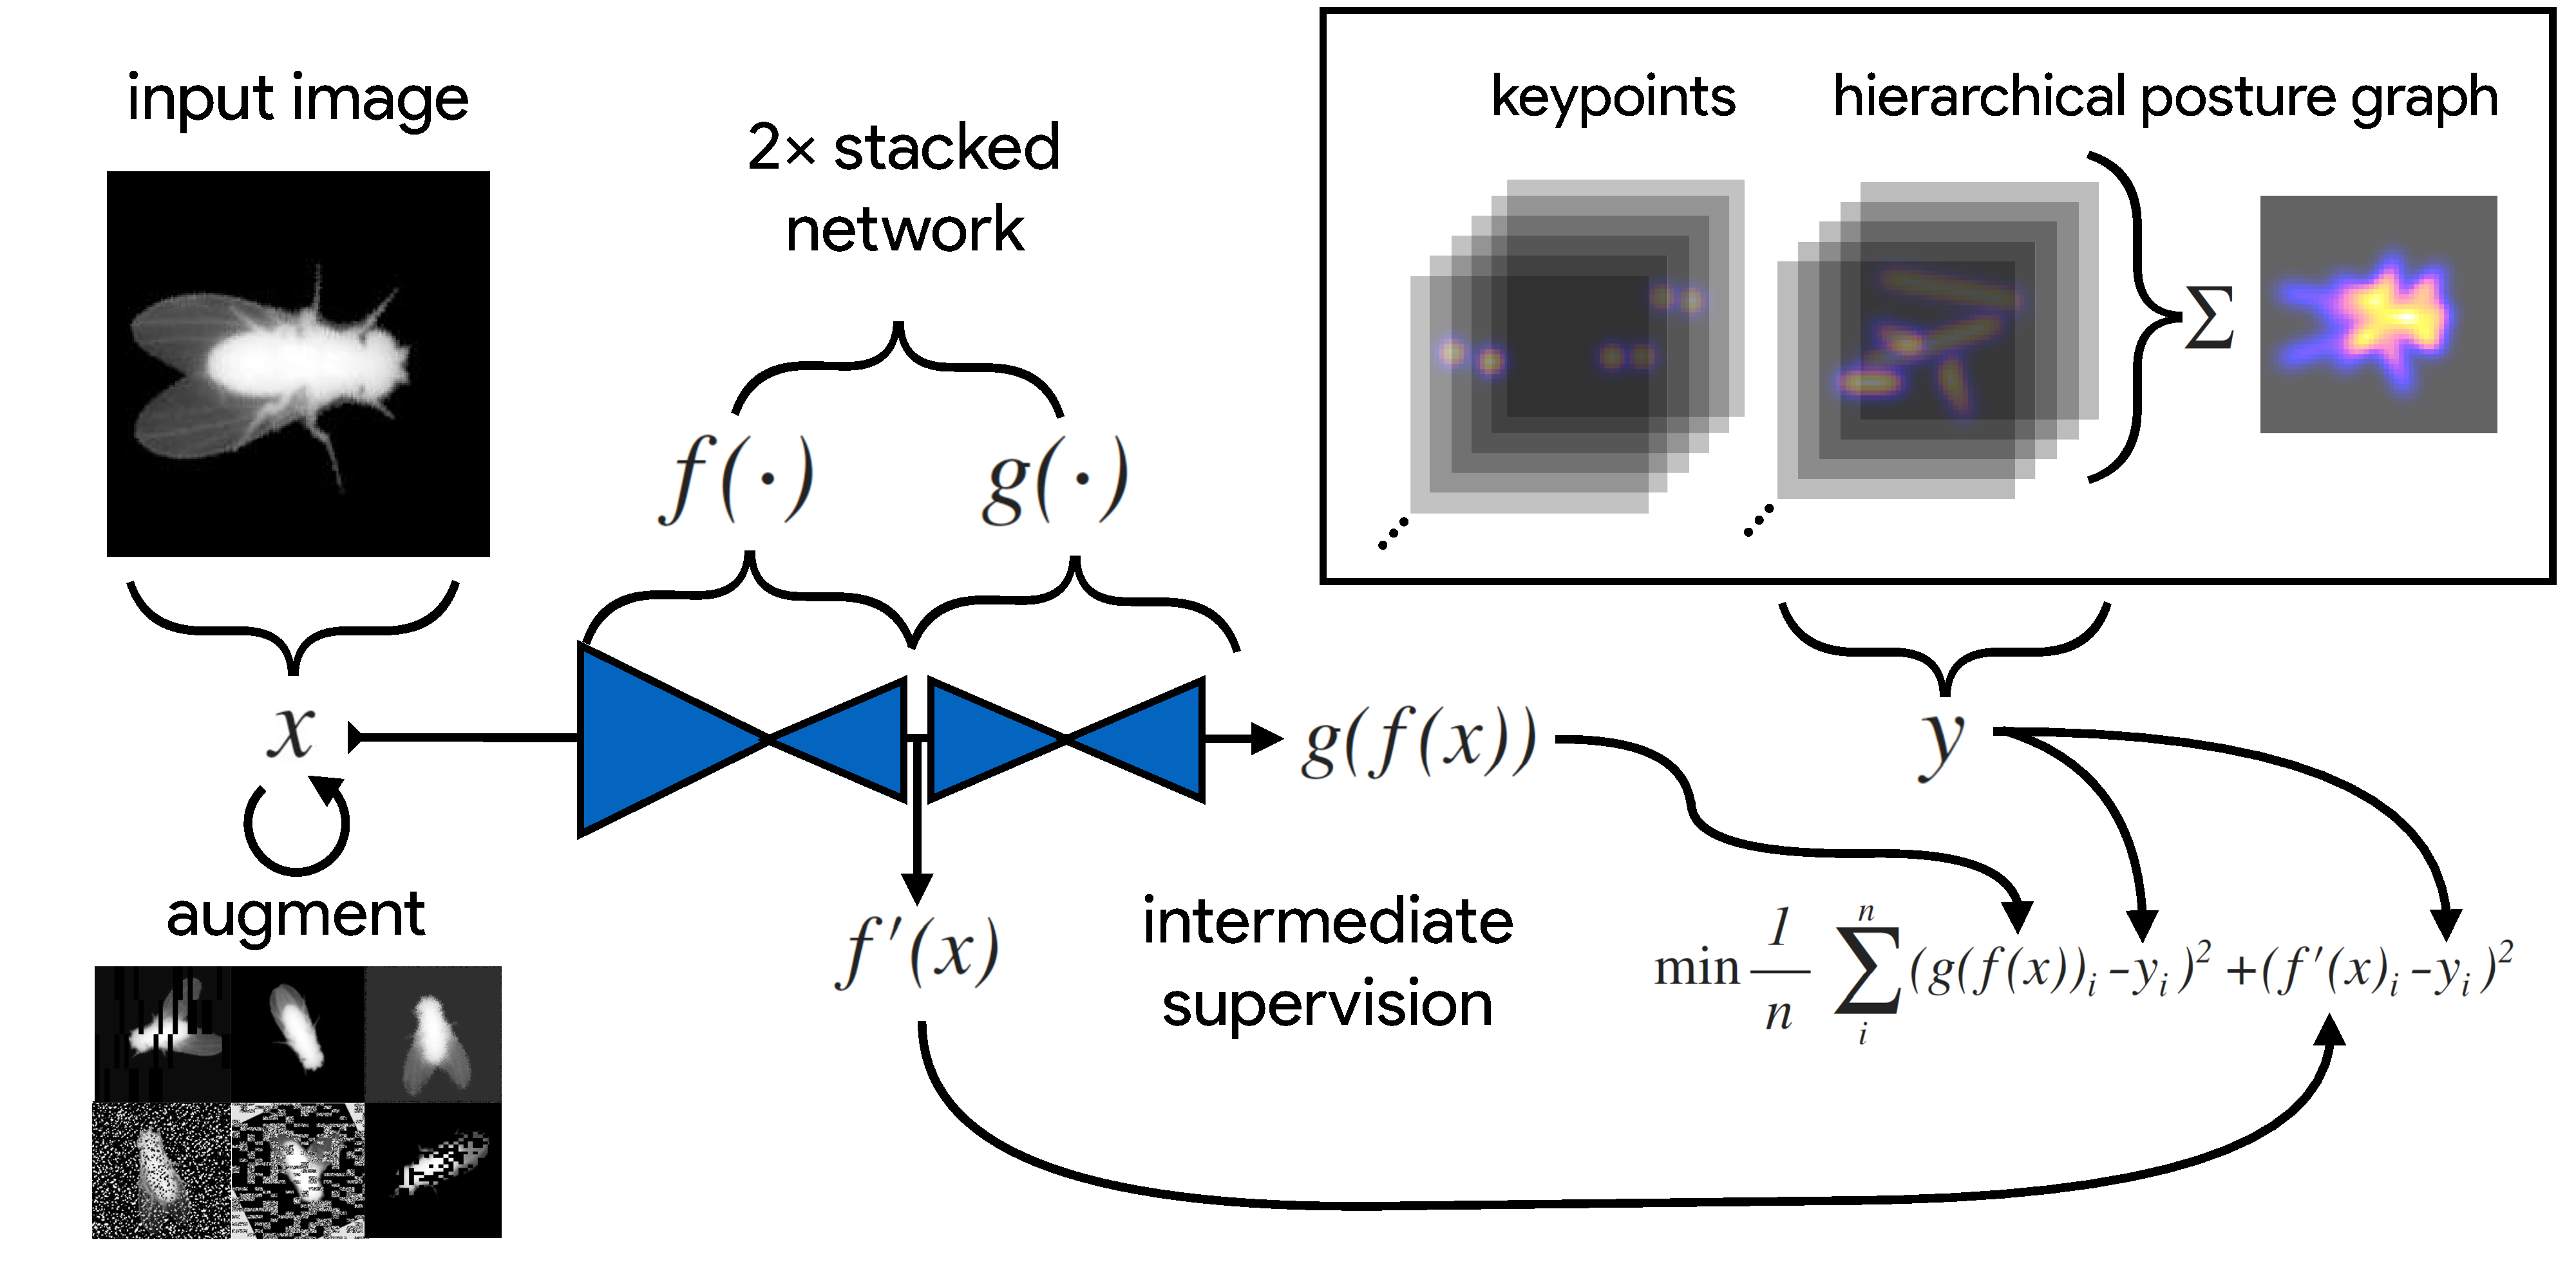
\includegraphics[width=0.95\linewidth]{Graving_IMPRS_Thesis/figures/model_training_figure.pdf}
\caption{An illustration of the model training process for our Stacked DenseNet model in DeepPoseKit (see Appendix \ref{app:cnn} for details about training models). Input images $x$ (\textbf{top-left}) are augmented (\textbf{bottom-left}) with various spatial transformations (rotation, translation, scale, etc.) followed by noise transformations (dropout, additive noise, blurring, contrast, etc.) to improve the robustness and generalization of the model. The ground truth annotations are then transformed with matching spatial augmentations (not shown for the sake of clarity) and used to draw the confidence maps $y$ for the keypoints and hierarchical posture graph (\textbf{top-right}). The images $x$ are then passed through the network to produce a multidimensional array $g(f(x))$—a stack of images corresponding to the keypoint and posture graph confidence maps for the ground truth $y$. Mean squared error between the outputs for both networks $g(f(x))$ and $f^{\prime}(x)$ and the ground truth data $y$ is then minimized (\textbf{bottom-right}), where $f^{\prime}(x)$ indicates a subset of the output from $f(x)$—only those feature maps being optimized to reproduce the confidence maps for the purpose of intermediate supervision (Appendix \ref{app:sota}). The loss function is minimized until the validation loss stops improving—indicating that the model has converged or is starting to overfit to the training data.}
\label{fig:model_training_figure}

\end{figure}


\subsection{An end-to-end pose estimation framework}
We provide a full-featured, extensible, and easy-to-use software package that is written entirely in the Python programming language (Python Software Foundation) and is built on the popular Keras deep-learning package \citep{chollet2015keras}—using TensorFlow as a backend \citep{tensorflow2015-whitepaper}. Our software is a complete, end-to-end pipeline (Figure \ref{fig:workflow_figure}) with a custom GUI for creating annotated training data with active learning similar to \citeauthor{pereira2019fast} (\citeyear{pereira2019fast}; Appendix \ref{app:training_data}), as well as a flexible pipeline for data augmentation (\citealt{jung2018imgaug}; Appendix \ref{app:training_data}; shown in Figure \ref{fig:model_training_figure}), model training and evaluation (Figure \ref{fig:model_training_figure}; Appendix \ref{app:cnn}), and running inference on new data. We designed our high-level programming interface using the same guidelines from Keras \citep{chollet2015keras} to allow the user to go from idea to result as quickly as possible, and we organized our software into a Python module called \textit{DeepPoseKit}. The code, documentation, and examples for our entire software package are freely available at \url{https://github.com/jgraving/deepposekit} under a permissive open-source license. 


\subsection{Our pose estimation models}
To achieve the goal of “fast animal pose estimation” introduced by \cite{pereira2019fast}, while maintaining the robust predictive power of models like DeepLabCut \citep{mathis2018deeplabcut}, we implemented two fast pose estimation models that extend the state-of-the-art model for individual pose estimation introduced by \cite{newell2016} and the current state-of-the art for convolutional regression from \cite{Jegou16}. Our model implementations use fewer parameters than both the DeepLabCut model \citep{mathis2018deeplabcut} and LEAP model \citep{pereira2019fast} while simultaneously removing many of the limitations of these architectures. 

In order to limit overparameterization while minimizing performance loss, we designed our models to allow for multi-scale inference (Appendix \ref{app:fcnn} Box \ref{box:encoder_decoder_box}) while optimizing our model hyperparameters for efficiency. Our first model is a novel implementation of \textit{FC-DenseNet} from \citeauthor{Jegou16} (\citeyear{Jegou16}; Appendix \ref{app:fcnn} Box \ref{box:encoder_decoder_box}) arranged in a stacked configuration similar to \citeauthor{newell2016} (\citeyear{newell2016}; Appendix \ref{app:sota}). We call this new model Stacked DenseNet, and to the best of our knowledge, this is the first implementation of this model architecture in the literature—for pose estimation or otherwise. Further details for this model are available in Appendix \ref{app:implementation}. Our second model is a modified version of the \textit{Stacked Hourglass} model from \citeauthor{newell2016} (\citeyear{newell2016}; Appendix \ref{app:sota}) with hyperparameters that allow for changing the number of filters in each convolutional block to constrain the number of parameters—rather than using 256 filters for all layers as described in \cite{newell2016}.

\subsection[Subpixel keypoint prediction on the GPU]{Subpixel keypoint prediction on the GPU allows for fast and accurate inference}
In addition to implementing our efficient pose estimation models, we developed a new method to process model outputs to allow for faster, more accurate predictions. When using a fully-convolutional posture estimation model, the confidence maps produced by the model must be converted into coordinate values for the predictions to be useful, and there are typically two choices for making this conversion. The first is to move the confidence maps out of GPU memory and post-process them on the CPU. This solution allows for easy, flexible, and accurate calculation of the coordinates with subpixel precision \citep{insafutdinov2016deepercut, mathis2018deeplabcut}. However, CPU processing is not ideal because moving large arrays of data between the GPU and CPU can be costly, and computation on the CPU is generally slower. The other option is to directly process the confidence maps on the GPU and then move the coordinate values from the GPU to the CPU. This approach usually means converting confidence maps to integer coordinates based on the row and column index of the global maximum for each confidence map \citep{pereira2019fast}. However, this means that, to achieve a precise estimation, the confidence maps should be predicted at the full resolution of the input image, or larger, which slows down inference speed.

As an alternative to these two strategies, we introduce a new GPU-based convolutional layer that we call \textit{subpixel maxima}. This layer uses the fast, efficient, image registration algorithm introduced by \cite{guizar2008efficient} to translationally align a centered two-dimensional Gaussian filter to each confidence map via Fourier-based convolution. The translational shift between the filter and each confidence map allows us to calculate the coordinates of the global maxima with high speed and subpixel precision. This technique allows for accurate predictions of keypoint locations even if the model's confidence maps are dramatically smaller than the resolution of the input image. We compared the accuracy of our subpixel maxima layer to an integer-based maxima layer using the fly dataset from \cite{pereira2019fast} (see "Methods"). We found significant accuracy improvements across every downsampling configuration (Appendix \ref{app:figures} Figure \ref{fig:downsample_inference_speed}a). Even with confidence maps at $\tfrac{1}{8}\times$ the resolution of the original image, error did not drastically increase compared to full-resolution predictions. Making predictions for confidence maps at such a downsampled resolution allows us to achieve very fast inference >1000 Hz while maintaining high accuracy (Appendix \ref{app:figures} Figure \ref{fig:downsample_inference_speed}b).

We also provide speed comparisons with the other models we tested and find that our Stacked DenseNet model with our subpixel peak detection algorithm is faster than the DeepLabCut model \citep{mathis2018deeplabcut} for both offline (batch size = 100) and real-time speeds (batch size = 1). While we find that our Stacked DenseNet model is faster than the LEAP model \citep{pereira2019fast} for offline processing (batch size = 100), the LEAP model \citep{pereira2019fast} is significantly faster for real-time processing (batch size = 1). Our Stacked Hourglass model \citep{newell2016} is about the same or slightly faster than Stacked DenseNet for offline speeds (batch size = 100), but is much slower for real-time processing (batch size = 1). Achieving fast pose estimation using CNNs typically relies on massively parallel processing on the GPU with large batches of data or requires downsampling the images to increase speed, which increases error \citep{mathis2018inference}. These factors make fast and accurate real-time inference challenging to accomplish. Our Stacked DenseNet model, with a batch size of one, can run inference at $\sim$30-110Hz—depending on the resolution of the predicted confidence maps (Appendix \ref{app:figures} Figure \ref{fig:downsample_inference_speed}b). These speeds are faster than the DeepLabCut model \citep{mathis2018deeplabcut} and could be further improved by downsampling the input image resolution or reconfiguring the model with fewer parameters. This allows our methods to be flexibly used for real-time or closed-loop behavioral experiments with prediction errors similar to current state-of-the-art methods. 


\subsection[Learning multi-scale geometry between keypoints improves accuracy]{Learning multi-scale geometry between keypoints improves accuracy and reduces extreme errors}

Minimizing extreme prediction errors is important to prevent downstream effects on any further behavioral analysis \citep{seethapathi2019movement}---especially in the case of analyses based on time-frequency transforms like those from \cite{berman2014mapping, berman2016predictability, klibaite2017unsupervised, todd2017systematic, klibaite2019interacting} and \cite{pereira2019fast} where high magnitude errors can cause inaccurate behavioral classifications. While effects of these extreme errors can be minimized using post-hoc filters and smoothing, these post-processing techniques can remove relevant high-frequency information from time-series data, so this solution is less than ideal. One way to minimize extreme errors when estimating posture is to incorporate multiple spatial scales when making predictions (e.g., \citealt{chen2017adversarial}). Our pose estimation models are implicitly capable of using information from multiple scales (see Appendix \ref{app:fcnn} Box \ref{box:encoder_decoder_box}), but there is no explicit signal that optimizes the model to take advantage of this information when making predictions.

To remedy this, we modified the model's output to predict, in addition to keypoint locations, a hierarchical graph of edges describing the multi-scale geometry between keypoints—similar to the part affinity fields described by \cite{cao2017realtime}. This was achieved by adding an extra set of confidence maps to the output where edges in the postural graph are represented by Gaussian-blurred lines the same width as the Gaussian peaks in the keypoint confidence maps. Our posture graph output then consists of four levels: (1) a set of confidence maps for the smallest limb segments in the graph (e.g., foot to ankle, knee to hip, etc.; Figure \ref{fig:model_training_figure}), (2) a set of confidence maps for individual limbs (e.g., left leg, right arm, etc.; Figure \ref{fig:posture_confidence_map_figure}), (3) a map with the entire postural graph, and (4) a fully-integrated map that incorporates the entire posture graph and confidence peaks for all of the joint locations (Figure \ref{fig:model_training_figure}). Each level of the hierarchical graph is built from lower levels in the output, which forces the model to learn correlated features across multiple scales when making predictions.

 We find that training our Stacked DenseNet model to predict a hierarchical posture graph reduces keypoint prediction error (Appendix \ref{app:figures} Figure \ref{fig:graph_error_figure}), and because the feature maps for the posture graph can be removed from the final output during inference, this effectively improves prediction accuracy for free. Both the mean and variance of the error distributions were lower when predicting the posture graph, which suggests that learning multi-scale geometry both decreases error on average and helps to reduce extreme prediction errors. The overall effect size for this decrease in error is fairly small (<1 pixel average reduction in error), but based on the results from the zebra dataset, this modification more dramatically improves performance for datasets with higher-variance images and sparse posture graphs. Predicting the posture graph may be especially useful for animals with long slender appendages such as insect legs and antennae where prediction errors are likely to occur due to occlusions and natural variation in the movement of these body parts. These results also suggest that annotating multiple keypoints to incorporate an explicit signal for multi-scale information may help improve prediction accuracy for a specific body part of interest.

\subsection{Stacked DenseNet is fast and robust}
\label{subsec:models}
We benchmarked our new model implementations against the models \citep{pereira2019fast} and \cite{mathis2018deeplabcut}. We find that our Stacked DenseNet model outperforms both the LEAP model \citep{pereira2019fast} and the DeepLabCut model \citep{mathis2018deeplabcut} in terms of speed while also achieving much higher accuracy than the LEAP model \citep{pereira2019fast} with similar accuracy to the DeepLabCut model (\citealt{mathis2018deeplabcut}; Figure \ref{fig:speed_accuracy_api}a). We found that both the Stacked Hourglass and Stacked DenseNet models outperformed the LEAP model \citep{pereira2019fast}. Notably our Stacked DenseNet model achieved approximately 2$\times$ faster inference speeds with 3$\times$ higher mean accuracy. Not only were our models’ average prediction error significantly improved, but also, importantly, the variance was lower—indicating that our models produced fewer extreme prediction errors. At $\tfrac{1}{4}\times$ resolution, our Stacked DenseNet model consistently achieved prediction accuracy nearly identical to the DeepLabCut model \citep{mathis2018deeplabcut} while running inference at nearly 2$\times$ the speed and using only $\sim$5$\%$ of the parameters—$\sim$1.5 million vs. $\sim$26 million. Detailed results of our model comparisons are shown in Figure \ref{fig:speed_accuracy_api}-Figure supplement \ref{figsupp:model_posterior_comparisons}.

While the Stacked DenseNet model used for comparisons is already fast, inference speed could be further improved by using a $\tfrac{1}{8}\times$ output without much increase in error (Appendix \ref{app:figures} Figure \ref{fig:downsample_inference_speed}) or by further adjusting the hyperparameters to constrain the size of the model. Our Stacked Hourglass implementation followed closely behind the performance of our Stacked DenseNet model and the DeepLabCut model \citep{mathis2018deeplabcut} but consistently performed more poorly than our Stacked DenseNet model in terms of prediction accuracy, so we excluded this model from further analysis. We were also able to reproduce the results reported by \cite{pereira2019fast} that the LEAP model and the Stacked Hourglass model \citep{newell2016} have similar average prediction error for the fly dataset. However, we also find that the LEAP model \citep{pereira2019fast} has much higher variance, which suggests it is more prone to extreme prediction errors—a problem for further data analysis.

\subsection{Stacked DenseNet trains quickly and requires few training examples}
To further compare models, we used our zebra dataset to assess the training time needed for our Stacked DenseNet model, the DeepLabCut model \citep{mathis2018deeplabcut}, and the LEAP model \citep{pereira2019fast} to reach convergence as well as the amount of training data needed for each model to generalize to new data from outside the training set. We find that our Stacked DenseNet model, the DeepLabCut model \citep{mathis2018deeplabcut}, and the LEAP model \citep{pereira2019fast} all fully converge in just a few hours and reach reasonably high accuracy after only an hour of training (Appendix \ref{app:figures} Figure \ref{fig:training_time}). However, it appears that our Stacked DenseNet model tends to converge to a good minimum faster than both the DeepLabCut model \citep{mathis2018deeplabcut} and the LEAP model \citep{pereira2019fast}.

We also show that our Stacked DenseNet model achieves good generalization with few training examples and without the use of transfer learning (Appendix \ref{app:figures} Figure \ref{fig:training_prop}). These results demonstrate that, when combined with data augmentation, as few as five training examples can be used as an initial training set for labelling keypoints with active learning (Figure \ref{fig:workflow_figure}). Additionally, because our analysis shows that generalization to new data plateaus after approximately 100 labeled training examples, it appears that 100 training examples is a reasonable minimum size for a training set---although the exact number will likely change depending the variance of the image data being annotated. To further examine the effect of transfer learning on model generalization, we compared performance between the DeepLabCut model \citep{mathis2018deeplabcut} initialized with weights pretrained on the ImageNet database \citep{deng2009imagenet} vs. the same model with randomly-initialized weights (Appendix \ref{app:figures} Figure \ref{fig:training_prop}). As postulated by \cite{mathis2018deeplabcut}, we find that transfer learning does provide some benefit to the DeepLabCut model's ability to generalize. However, the effect size of this improvement is small with a mean reduction in Euclidean error of <0.5 pixel. Together these results indicate that transfer learning is helpful, but not required, for deep learning models to achieve good generalization with limited training data.

\begin{figure}[!htb]

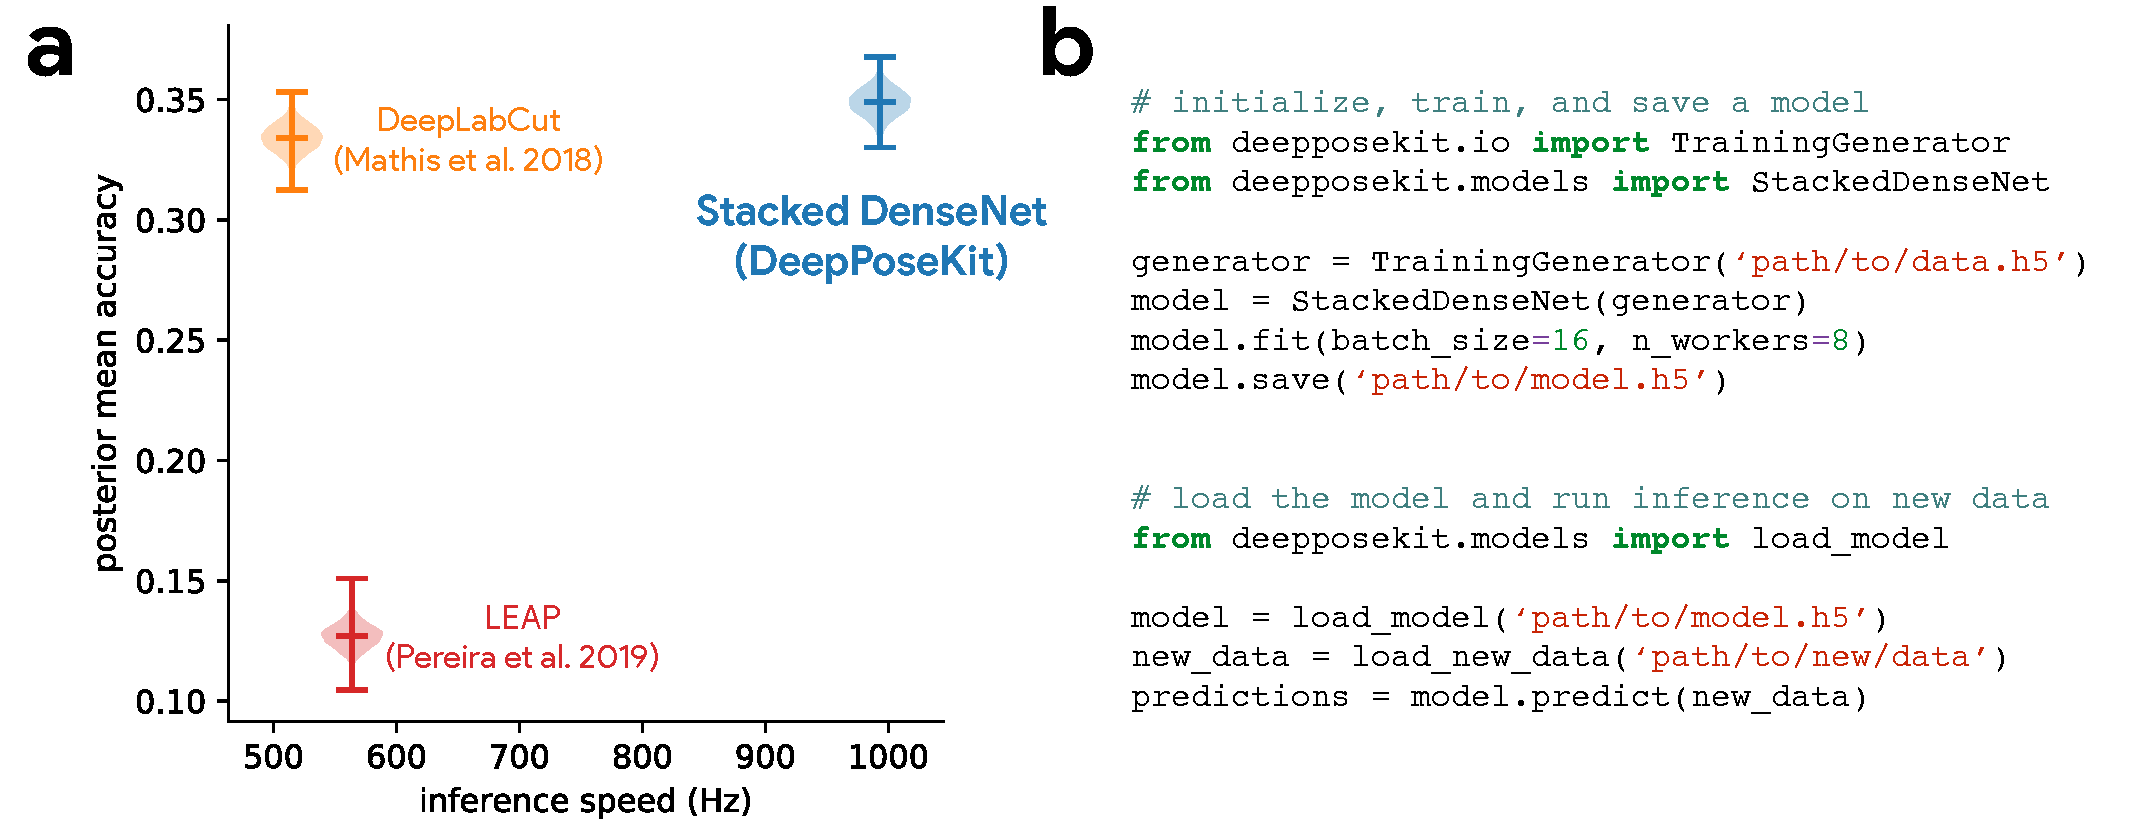
\includegraphics[width=0.95\linewidth]{Graving_IMPRS_Thesis/figures/speed_accuracy_api_figure.pdf}
\caption{Our Stacked DenseNet model estimates posture at approximately 2$\times$—or greater—the speed of the LEAP model \citep{pereira2019fast} and the DeepLabCut model \citep{mathis2018deeplabcut} while also achieving similar accuracy to the DeepLabCut model \citep{mathis2018deeplabcut}—shown here as mean accuracy $(1 + \textrm{Euclidean error})^{-1}$ for our most challenging dataset of multiple interacting Grévy's zebras (\textit{E. grevyi}) recorded in the wild (\textbf{a}). See Figure \ref{fig:speed_accuracy_api} supplement \ref{figsupp:model_posterior_comparisons} for further details. Our software interface is designed to be straightforward but flexible. We include many options for expert users to customize model training with sensible default settings to make pose estimation as easy as possible for beginners. For example, training a model and running inference on new data requires writing only a few lines of code and specifying some basic settings (\textbf{b}).}
\label{fig:speed_accuracy_api}
%\figdata{Raw prediction errors used for model comparisons in Figure \ref{fig:speed_accuracy_api}-Figure supplement \ref{figsupp:model_posterior_comparisons}. See "Methods" for details.}\label{figdata:model_comparisons}


\end{figure}
\begin{figure}[!htb]
    \centering
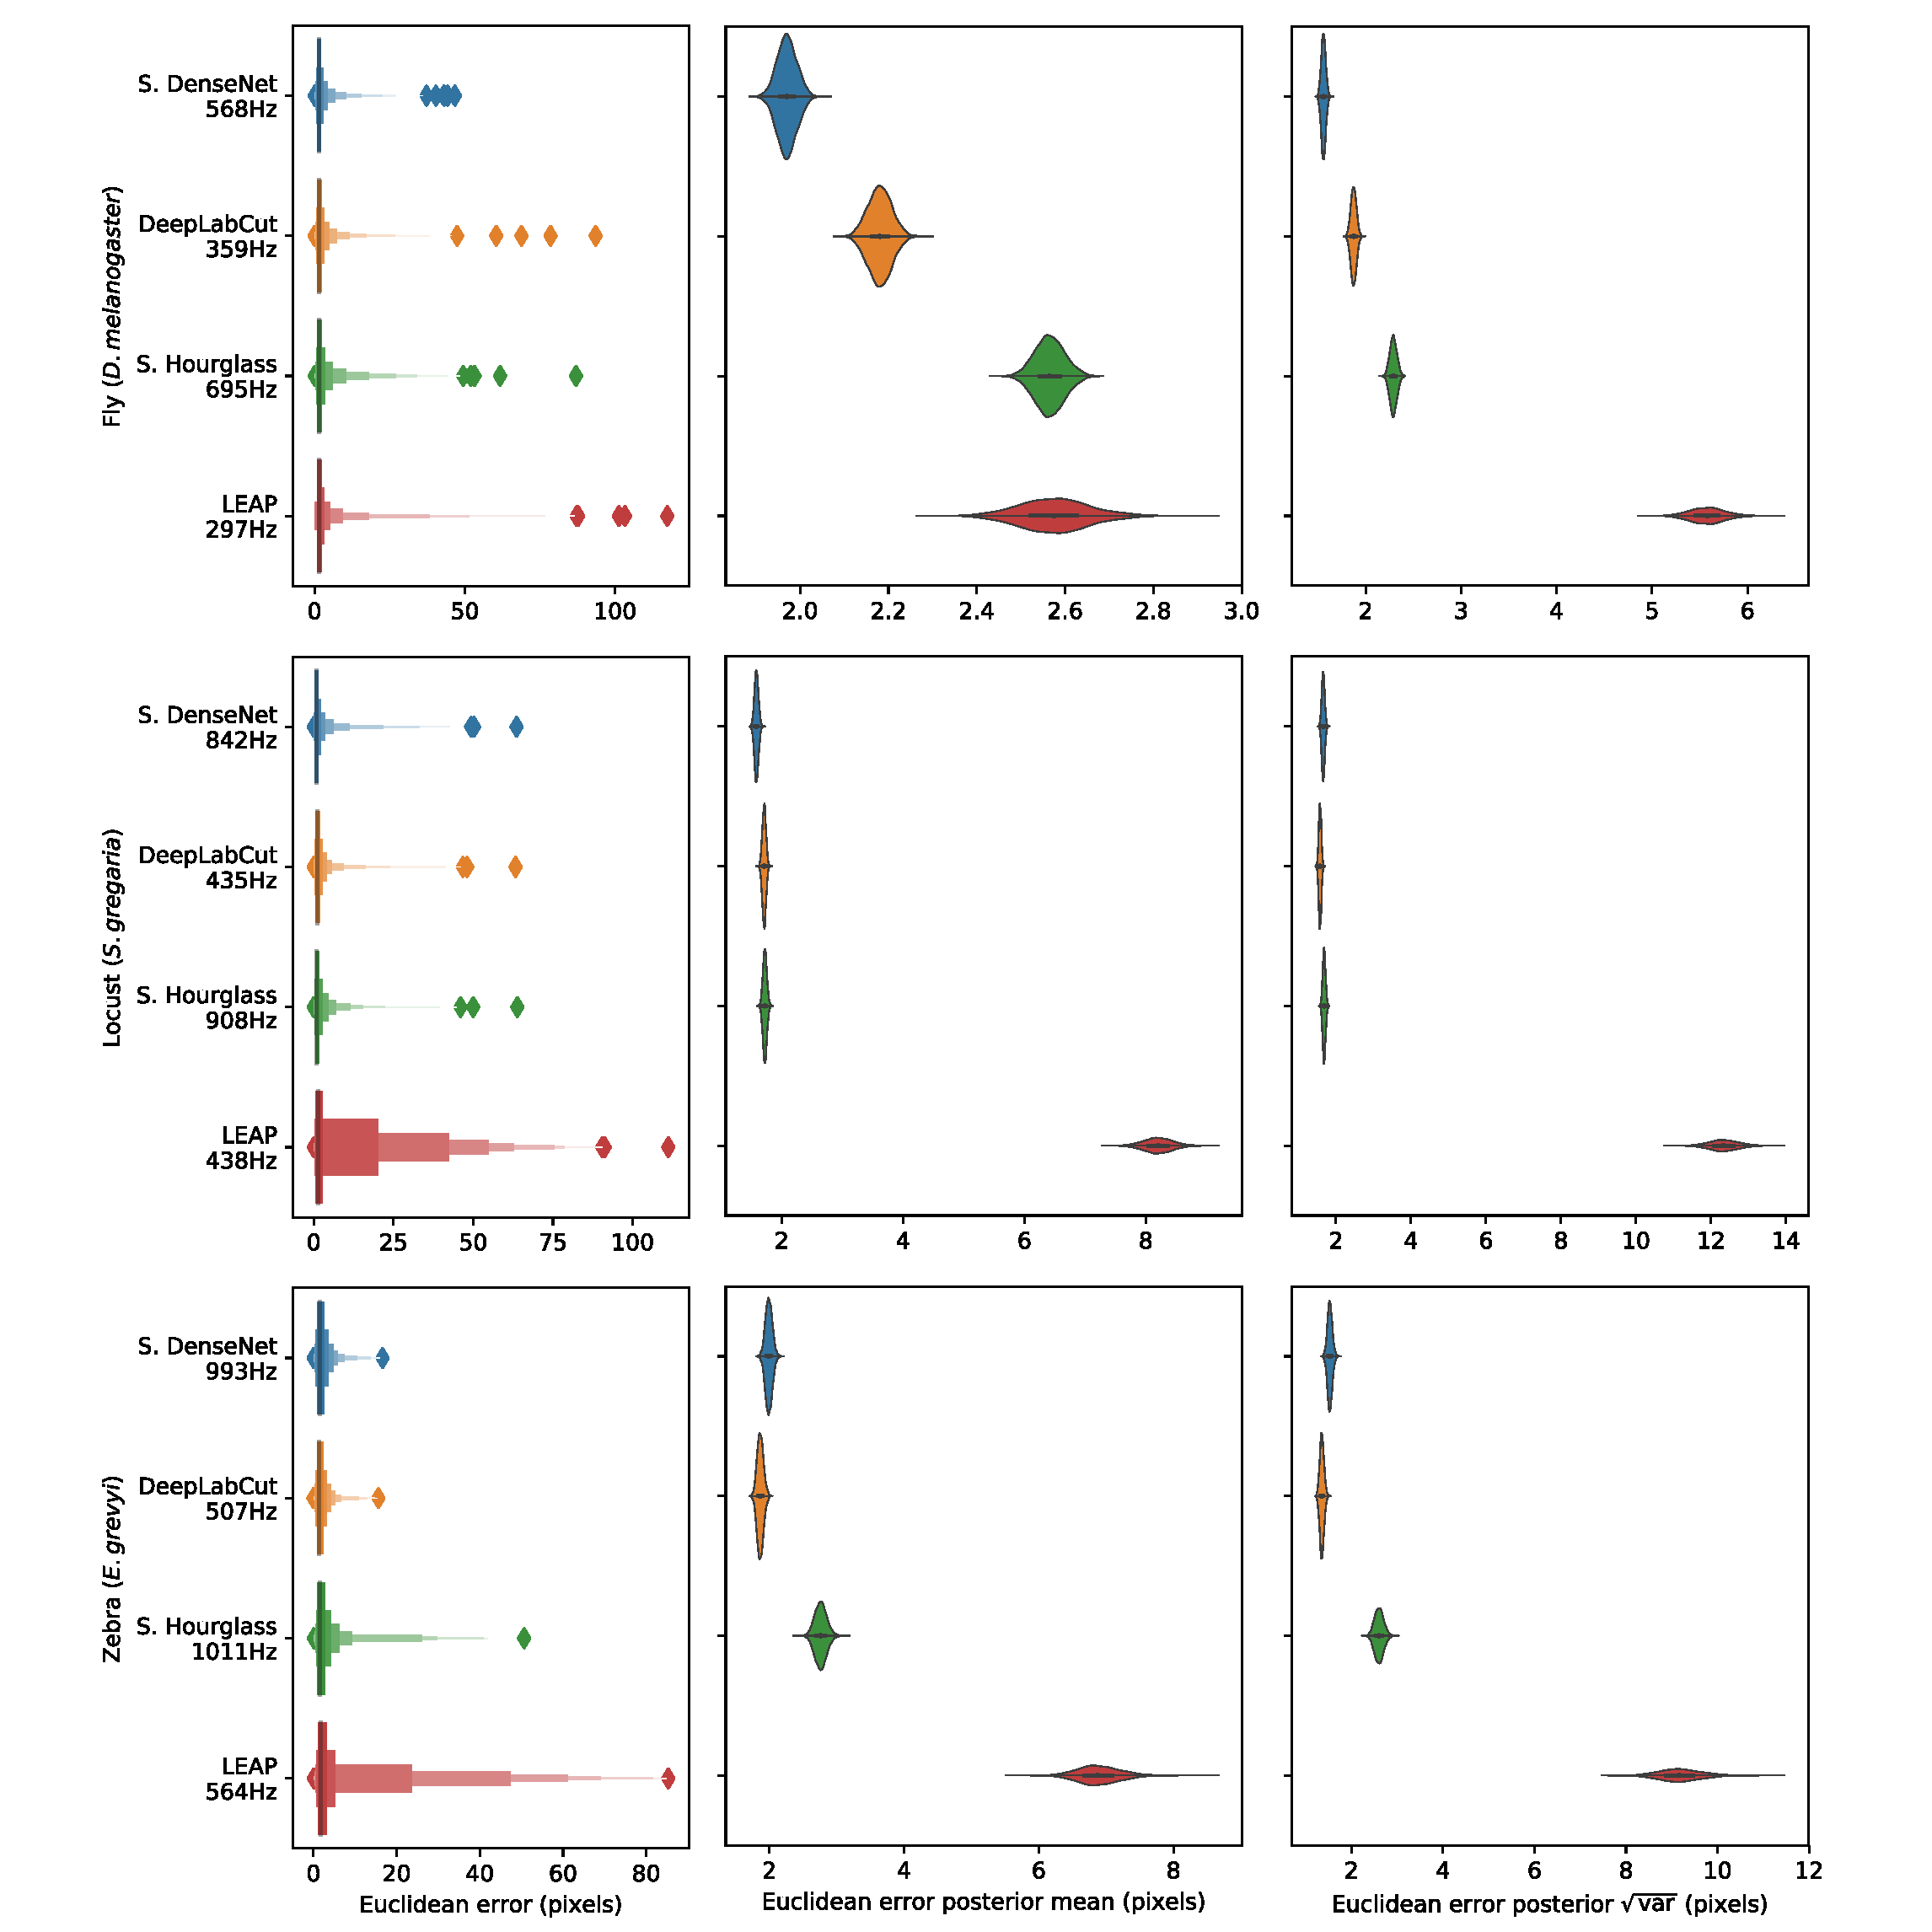
\includegraphics[width=\linewidth]{Graving_IMPRS_Thesis/figures/model_posteriors_figure.pdf}
\caption{Euclidean error distributions for each model across our three datasets. Letter-value plots (\textbf{left}) show the raw error distributions for each model. Violinplots of the posterior distributions for the mean and variance (\textbf{right}) show statistical differences between the error distributions. Overall the LEAP model \citep{pereira2019fast} was the worst performer on every dataset in terms of both mean and variance. Our Stacked Densenet model was the best performer for the fly dataset, while our Stacked DenseNet model and the DeepLabCut model \citep{mathis2018deeplabcut} both performed equally well on the locust and zebra datasets. The posteriors for the DeepLabCut model \citep{mathis2018deeplabcut} and our Stacked DenseNet model are highly overlapping for these datasets, which suggests they are not statistically discernible from one another. Our Stacked Hourglass model \citep{newell2016} performed equally to the DeepLabCut model \citep{mathis2018deeplabcut} and our Stacked DenseNet model for the locust dataset but performed slightly worse for the fly and zebra datasets.}
\label{figsupp:model_posterior_comparisons}
\end{figure}


\section{Discussion}
Here we have presented a new software toolkit, called DeepPoseKit, for estimating animal posture using deep learning models. We built on the state-of-the-art for individual pose estimation using convolutional neural networks to achieve fast inference without reducing accuracy or generalization ability. Our new pose estimation model, called Stacked DenseNet, offers considerable improvements (Figure \ref{fig:speed_accuracy_api}a; Figure supplement \ref{figsupp:model_posterior_comparisons}) over the models from \cite{mathis2018deeplabcut} (DeepLabCut) and \cite{pereira2019fast} (LEAP), and our software framework also provides a simplified interface (Figure \ref{fig:speed_accuracy_api}b) for using these advanced tools to measure animal behavior and locomotion. We tested our methods across a range of datasets from controlled laboratory environments with single individuals to challenging field situations with multiple interacting individuals and variable lighting conditions. We found that our methods perform well for all of these situations and require few training examples to achieve good predictive performance on new data---without the use of transfer learning. We ran experiments to optimize our approach and discovered that some straightforward modifications can greatly improve speed and accuracy. Additionally, we demonstrated that these modifications improve not the just the average error but also help to reduce extreme prediction errors—a key determinant for the reliability of subsequent statistical analysis.

While our results offer a good-faith comparison of the available methods for animal pose estimation, there is inherent uncertainty that we have attempted to account for but may still bias our conclusions. For example, deep learning models are trained using stochastic optimization algorithms that give different results with each replicate, and the Bayesian statistical methods we use for comparison are explicitly probabilistic in nature. There is also great variability across hardware and software configurations when using these models in practice \citep{mathis2018inference}, so performance may change across experimental setups and datasets. Additionally, we demonstrated that some models may perform better than others for specific applications (Figure \ref{fig:speed_accuracy_api} supplement \ref{figsupp:model_posterior_comparisons}), and to account for this, our toolkit offers researchers the ability to choose the model that best suits their requirements—including the LEAP model \citep{pereira2019fast} and the DeepLabCut model \citep{mathis2018deeplabcut}.  

We highlighted important considerations when using CNNs for pose estimation and reviewed the progress of fully-convolutional regression models from the literature. The latest advancements for these models have been driven mostly by a strategy of adding more connections between layers to increase performance and efficiency (e.g., \citealt{Jegou16}). Future progress for this class of models may require better loss functions \citep{goodfellow2014generative, johnson2016perceptual, chen2017adversarial, zhang2018unreasonable} that more explicitly model the spatial dependencies within a scene, models that incorporate the temporal structure of the data \citep{seethapathi2019movement}, and more mathematically-principled approaches (e.g., \citealt{weigert2018content, roy2018bayesian}) such as the application of formal probabilistic concepts \citep{kendall2017uncertainties} and Bayesian inference at scale \citep{tran2018simple}. 

Measuring behavior is a critical factor for many studies in neuroscience \citep{krakauer2017neuroscience}. Understanding the connections between brain activity and behavioral output requires detailed and objective descriptions of body posture that match the richness and resolution neural measurement technologies have provided for years \citep{anderson2014toward,berman2018measuring,brown2018ethology}, which our methods and other deep-learning–based tools provide \citep{mathis2018deeplabcut, pereira2019fast}. We have also demonstrated the possibility that our toolkit could be used for real-time inference, which allows for closed-loop experiments where sensory stimuli or optogenetic stimulation are controlled in response to behavioral measurements (e.g., \citealt{bath2014flymad,stowers2017virtual}). Using real-time measurements in conjunction with optogenetics or thermogenetics may be key to disentangling the causal structure of motor output from the brain—especially given that recent work has shown an animal's response to optogenetic stimulation can differ depending on the behavior it is currently performing \citep{cande2018optogenetic}. Real-time behavioral quantification is also particularly important as closed-loop virtual reality is quickly becoming an indispensable tool for studying sensorimotor relationships in individuals and collectives \citep{stowers2017virtual}. 

Quantifying individual movement is essential for revealing the genetic \citep{kain2012phototactic, brown2013dictionary, ayroles2015behavioral} and environmental \citep{bierbach2017behavioural, akhund2019effect, versace2019individual} underpinnings of phenotypic variation in behavior—as well as the phylogeny of behavior (e.g., \citealt{berman2014mappingv1}). Measuring individual behavioral phenotypes requires tools that are robust, scaleable, and easy-to-use, and our approach offers the ability to quickly and accurately quantify the behavior of many individuals in great detail. When combined with tools for genetic manipulations \citep{ran2013genome,doudna2014new}, high-throughput behavioral experiments \citep{alisch2018maple, javer2018open, werkhoven2019margo}, and behavioral analysis (e.g., \citealt{berman2014mapping, wiltschko2015mapping}), our methods could help to provide the data resolution and statistical power needed for dissecting the complex relationships between genes, environment, and behavioral variation.

When used together with other tools for localization and tracking (e.g., \citealt{perez2014idtracker, crall2015beetag, graving2017pinpoint, romero2018idtracker, wild2018honeybee,boenisch2018tracking}), our methods are capable of reliably measuring posture for multiple interacting individuals. The importance of measuring detailed representations of individual behavior when studying animal collectives has been well established \citep{strandburg2013visual,rosenthal2015revealing,strandburg2015shared,strandburg2017habitat}. Estimating body posture is an essential first step for unraveling the sensory networks that drive group coordination, such as vision-based networks measured via raycasting \citep{strandburg2013visual,rosenthal2015revealing}. Additionally, using body pose estimation in combination with computational models of behavior (e.g., \citealt{Costa1501}, \citealt{wiltschko2015mapping}) and unsupervised behavioral classification methods (e.g., \citealt{berman2014mapping}, \citealt{pereira2019fast}) may allow for further dissection of how information flows through groups by revealing the networks of behavioral contagion across multiple timescales and sensory modalities. While we have provided a straightforward solution for applying existing pose estimation methods to measure collective behavior, there still remain many challenging scenarios where these methods would fail. For example, tracking posture in a densely-packed bee hive or school of fish would require novel solutions to deal with the 3-D nature of individual movement, which includes maintaining individual identities and dealing with the resulting occlusions that go along with imaging these types of biological systems.  

When combined with unmanned aerial vehicles (UAVs; \citealt{schiffman2014drones}) or other field-based imaging \citep{francisco2020high}, applying these methods to the study of individuals and groups in the wild can provide high-resolution behavioral data that goes beyond the capabilities of current GPS and accelerometry-based technologies \citep{nagy2010hierarchical,nagy2013context,kays2015terrestrial,strandburg2015shared,strandburg2017habitat,flack2018local}—especially for species that are impractical to study with tags or collars. Additionally, by applying these methods in conjunction with 3-D habitat reconstruction—using techniques from photogrammetry  \citep{strandburg2017habitat, francisco2020high}—field-based studies can begin to integrate fine-scale behavioral measurements with the full 3-D environment in which the behavior evolved. Future advances will likely allow for the calibration and synchronizaton of imaging devices across multiple UAVs (e.g. \citealt{price2018deep, Nitin_ICCV_19}). This would make it possible to measure the full 3-D posture of wild animals (e.g. \citealt{Zuffi:ICCV:2019}) in scenarios where fixed camera systems (e.g. \citealt{nath2018}) would not be tractable, such as during migratory or predation events. When combined, these technologies could allow researchers to address questions about the behavioral ecology of animals that were previously impossible to answer.

Computer vision algorithms for measuring behavior at the scale of posture have rapidly advanced in a very short time; nevertheless, the task of pose estimation is far from solved. There are hard limitations to this current generation of pose estimation methods that are primarily related to the requirement for human annotations and user-defined keypoints---both in terms of the number of keypoints, the specific body parts being tracked, and the inherent difficulty of incorporating temporal information into the annotation and training procedure. Often the body parts chosen for annotation are an obvious fit for the experimental design and have reliably-visible reference points on the animal's body that make them easy to annotate. However, in many cases the required number and type of body parts needed for data analysis may not so obvious---such as in the case of unsupervised behavior classification methods \citep{berman2014mapping, pereira2019fast}. Additionally, the reference points for labeling images with keypoints can be hard to define and consistently annotate across images, which is often the case for soft or flexible-bodied animals like worms and fish. Moreover, due to the laborious nature of annotating keypoints, the current generation of methods also rarely takes into account the natural temporal structure of the data, instead treating each video frame as a statistically independent event, which can lead to extreme prediction errors (reviewed by \citealt{seethapathi2019movement}). Extending these methods to track the full three-dimensional posture of animals also typically requires the use of multiple synchronized cameras \citep{nath2018, gunel2019deepfly3d}, which increases the cost and complexity of creating an experimental setup, as well as the manual labor required for annotating a training set, which must include labeled data from every camera view.

These limitations make it clear that fundamentally-different methods may be required to move the field forward. Future pose estimation methods will likely replace human annotations with fully-articulated volumetric 3-D models of the animal's body (e.g., \citealt{zuffi20173d, Zuffi:ICCV:2019}), and the 3-D scene will be learned in an unsupervised or weakly-supervised way (e.g., \citealt{jaques2019physics, Zuffi:ICCV:2019}), where the shape, position, and posture of the animal's body, the camera position and lens parameters, and the background environment and lighting conditions will all be jointly learned directly from 2-D images by a deep-learning model \citep{ TensorflowGraphicsIO2019, Zuffi:ICCV:2019}. These \textit{inverse graphics models} \citep{kulkarni2015deep, sabour2017dynamic, TensorflowGraphicsIO2019} will likely take advantage of recently-developed differentiable graphics engines that allow 3-D rendering parameters to be straightforwardly controlled using computationally-efficient optimization methods \citep{Zuffi:ICCV:2019, TensorflowGraphicsIO2019}. After optimization, the volumetric 3-D timeseries data predicted by the deep learning model could be used directly for behavioral analysis or specific keypoints or body parts could be selected for analysis post-hoc. In order to more explicitly incorporate the natural statistical properties of the data, these models will also likely rely on the use of perceptual \citep{johnson2016perceptual, zhang2018unreasonable, Zuffi:ICCV:2019} and adversarial \citep{goodfellow2014generative, chen2017adversarial, kanazawa2019learning} loss functions that incorporate spatial dependencies within the scene rather than modeling each video frame as a set of statistically independent pixel distributions---as is the case with current methods that use factorized likelihood functions such as pixel-wise mean squared error (e.g., \citealt{pereira2019fast}) or cross-entropy loss (e.g., \citealt{mathis2018deeplabcut}). Because there would be limited or no requirement for human-provided labels, these models could also be easily modified to incorporate the temporal structure of the data using autoregressive representations (e.g., \citealt{van2016conditional, oord2016wavenet, kanazawa2019learning, kumar2019videoflow}), rather than modeling the scene in each video frame as a statistically independent event. Together these advances could lead to larger, higher-resolution, more reliable behavioral datasets that could revolutionize our understanding of relationships between behavior, the brain, and the environment.


In conclusion, we have presented a new toolkit, called DeepPoseKit, for automatically measuring animal posture from images. We combined recent advances from the literature to create methods that are fast, robust, and widely applicable to a range of species and experimental conditions. When designing our framework we emphasized usability across the entire software interface, which we expect will help to make these advanced tools accessible to a wider range of researchers. The fast inference and real-time capabilities of our methods should also help further reduce barriers to previously intractable questions across many scientific disciplines—including neuroscience, ethology, and behavioral ecology—both in the laboratory and the field.


\section{Methods}

We ran three main experiments to test and optimize our approach. First, we compared our new subpixel maxima layer to an integer-based global maxima with downsampled outputs ranging from 1$\times$ to $\tfrac{1}{16}\times$ the input resolution using our Stacked DenseNet model. Next, we tested if training our Stacked DenseNet model to predict the multi-scale geometry of the posture graph improves accuracy. Finally, we compared our model implementations of Stacked Hourglass and Stacked DenseNet to the models from \cite{pereira2019fast} (LEAP) and \cite{mathis2018deeplabcut} (DeepLabCut), which we also implemented in our framework (see Appendix \ref{app:implementation} for details). We assessed both the inference speed and prediction accuracy of each model as well as training time and generalization ability. When comparing these models we incorporated the relevant improvements from our experiments—including subpixel maxima and predicting multi-scale geometry between keypoints—unless otherwise noted (see Appendix \ref{app:implementation}).

While we do make comparisons to the DeepLabCut model \citep{mathis2018deeplabcut} we do not use the same training routine as \cite{mathis2018deeplabcut} and \cite{nath2018}, who use binary cross-entropy loss for optimizing the confidence maps in addition to the location refinement maps described by \cite{insafutdinov2016deepercut}. We made this modification in order to hold the training routine constant for each model while only varying the model itself. However, we find that these differences between training routines effectively have no impact on performance when the models are trained using the same dataset and data augmentations (Appendix \ref{app:implementation} Figure \ref{fig:dlc_comparison}). We also provide qualitative comparisons to demonstrate that, when trained with our DeepPoseKit framework, our implementation of the DeepLabCut model \citep{mathis2018deeplabcut} appears to produce fewer prediction errors than the original implementation from \cite{mathis2018deeplabcut, nath2018} when applied to a novel video (Appendix \ref{app:implementation} Figure \ref{fig:dlc_comparison}-Figure supplements \ref{figsupp:dlc_tsplot} and \ref{figsupp:dlc_dxtsplot}; Appendix \ref{app:implementation} Figure \ref{fig:dlc_comparison}-video \ref{videosupp:dlcsv1}). 


\subsection{Datasets}
We performed experiments using the vinegar or "fruit" fly (\textit{Drosophila melanogaster}) dataset (Figure \ref{fig:posture_confidence_map_figure}-video \ref{videosupp:sv1}) provided by \cite{pereira2019fast}, and to demonstrate the versatility of our methods we also compared model performance across two previously unpublished posture data sets from groups of desert locusts (\textit{Schistocerca gregaria}) recorded in a laboratory setting (Figure \ref{fig:posture_confidence_map_figure}-video \ref{videosupp:sv2}), and herds of Grévy's zebras (\textit{Equus grevyi}) recorded in the wild (Figure \ref{fig:posture_confidence_map_figure}-video \ref{videosupp:sv3}). The locust and zebra datasets are particularly challenging for pose estimation as they feature multiple interacting individuals—with focal individuals centered in the frame—and the latter with highly-variable environments and lighting conditions. These datasets are freely-available from \url{https://github.com/jgraving/deepposekit-data} \citep{graving2019data}.

Our locust dataset consisted of a group of 100 locusts in a circular plastic arena 1-m in diameter. The locust group was recorded from above using a high-resolution camera (Basler ace acA2040-90umNIR) and video recording system (Motif, loopbio GmbH). Locusts were localized and tracked using 2-D barcode markers \citep{graving2017pinpoint} attached to the thorax with cyanoacrylate glue, and any missing localizations ($<0.02 \%$ of the total dataset) between successful barcode reads were interpolated with linear interpolation.  Our zebra dataset consisted of variably sized groups in the wild recorded from above using a commercially-available quadcopter drone (DJI Phantom 4 Pro). Individual zebra were localized using custom deep-learning software based on Faster R-CNN \citep{ren2015faster} for predicting bounding boxes. The positions of each zebra were then tracked across frames using a linear assignment algorithm \citep{munkres1957algorithms} and data were manually verified for accuracy.

After positional tracking, the videos were then cropped using the egocentric coordinates of each individual and saved as separate videos---one for each individual. The images used for each training set were randomly selected using the k-means sampling procedure (with k=10) described by \cite{pereira2019fast} (Appendix \ref{app:training_data}) to reduce correlation between sampled images. After annotating the images with keypoints, we rotationally and translationally aligned the images and keypoints using the central body axis of the animal in each labeled image. This step allowed us to more easily perform data augmentations (see "Model training") that allow the model to make accurate predictions regardless of the animal's body size and orientation (see Appendix \ref{app:overparam}). However, this preprocessing step is not a strict requirement for training, and there is no requirement for this preprocessing step when making predictions on new unlabeled data, such as with the methods described by \cite{pereira2019fast} (Appendix \ref{app:overparam}). Before training each model we split each annotated dataset into randomly selected training and validation sets with 90\% training examples and 10\% validation examples, unless otherwise noted. The details for each dataset are described in Table \ref{tab:datasets}.

\begin{figure}[!htb]

\begin{center}
\includegraphics[width=0.9\linewidth]{Graving_IMPRS_Thesis/figures/posture_confidence_map_figure.pdf}
\end{center}
\caption{A visualization of the datasets we used to evaluate our methods (Table \ref{tab:datasets}). For each dataset, confidence maps for the keypoints (bottom-left) and posture graph (top-right) are illustrated using different colors for each map. These outputs are from our Stacked DenseNet model at $\frac{1}{4}\times$ resolution.}
\label{fig:posture_confidence_map_figure}


\end{figure}
\begin{figure}[!htb]
    \centering
    \caption{A video of a behaving fly from \cite{pereira2019fast} with pose estimation outputs visualized \url{https://youtu.be/lsnex6k4NRs}}
    \label{videosupp:sv1}
\end{figure}

\begin{figure}[!htb]
    \centering
    \caption{A video of a behaving locust with pose estimation outputs visualized. \url{https://youtu.be/b0DyyLP_Czk}}
    \label{videosupp:sv2}
\end{figure}

\begin{figure}[!htb]
    \centering
    \caption{A video of a behaving Grévy's zebra with pose estimation outputs visualized. \url{https://youtu.be/dSjaphoGHAY}}
    \label{videosupp:sv3}
\end{figure}


\begin{table}[!htb]

\caption{\label{tab:datasets}Datasets used for model comparisons.}
% Use "S" column identifier to align on decimal point 
\setlength{\tabcolsep}{2pt}
\centering
\begin{tabular}{|m{0.14\textwidth}|m{0.14\textwidth}|m{0.14\textwidth}|m{0.14\textwidth}|m{0.14\textwidth}|m{0.14\textwidth}|m{0.14\textwidth}|}
\hline
{Name} & Species   & {Resolution}  & {$\#$ Images}  & {$\#$ Keypoints} & {Individuals} & Source    \\ \hline
Vinegar fly  & \textit{Drosophila melanogaster} & {192$\times$192} & 1500 & 32 & Single & \cite{pereira2019fast} \\ \hline
Desert locust     & \textit{Schistocerca gregaria}       & 160$\times$160           & 800    & 35 & Multiple  & This paper\\ \hline
Grévy's zebra      & \textit{Equus grevyi}      & 160$\times$160              & 900    & 9 & Multiple & This paper \\ \hline
\end{tabular}

\end{table}

\subsection{Model training}
For each experiment, we set our model hyperparameters to the same configuration for our Stacked DenseNet and Stacked Hourglass models. Both models were trained with $\tfrac{1}{4}\times$ resolution outputs and a stack of two networks with two outputs where loss was applied (see Figure \ref{fig:model_training_figure}). Although our model hyperparameters could be infinitely adjusted to trade off between speed and accuracy, we compared only one configuration for each of our model implementations. These results are not meant to be an exhaustive search of model configurations as the best configuration will depend on the application. The details of the hyperparameters we used for each model are described in Appendix \ref{app:implementation}.

To make our posture estimation tasks closer to realistic conditions, incorporate prior information (Appendix \ref{app:training_data}), and properly demonstrate the robustness of our methods to rotation, translation, scale, and noise, we applied various augmentations to each data set during training (Figure \ref{fig:model_training_figure}). All models were trained using data augmentations that included random flipping, or mirroring, along both the horizontal and vertical image axes with each axis being independently flipped by drawing from a Bernoulli distribution (with $p=0.5$); random rotations around the center of the image drawn from a uniform distribution in the range [-180$\degree$, +180$\degree$); random scaling drawn from a uniform distribution in the range [90\%, 110\%] for flies and locusts and [75\%, 125\%] for zebras (to account for greater size variation in the data set); and random translations along the horizontal and vertical axis independently drawn from a uniform distribution with the range [-5\%, +5\%]---where percentages are relative to the original image size. After performing these spatial augmentations we also applied a variety of noise augmentations that included additive noise---i.e., adding or subtracting randomly-selected values to pixels; dropout---i.e., setting individual pixels or groups of pixels to a randomly-selected value; blurring or sharpening---i.e., changing the composition of spatial frequencies; and contrast ratio augmentations---i.e, changing the ratio between the highest pixel value and lowest pixel value in the image. These augmentations help to further ensure robustness to shifts in lighting, noise, and occlusions. See Appendix \ref{app:training_data} for further discussion on data augmentation.

We trained our models (Figure \ref{fig:model_training_figure}) using mean squared error loss optimized using the ADAM optimizer \citep{kingma2014adam} with a learning rate of $1\times10^{-3}$ and a batch size of 16. We lowered the learning rate by a factor of 5 each time the validation loss did not improve by more than $1\times10^{-3}$ for 10 epochs. We considered models to be converged when the validation loss stopped improving for 50 epochs, and we calculated validation error as the Euclidean distance between predicted and ground-truth image coordinates for only the best performing version of the model, which we evaluated at the end of each epoch during optimization. We performed this procedure five times for each experiment and randomly selected a new validation set for each replicate.

\subsection{Model evaluation}
Machine learning models are typically evaluated for their ability to generalize to new data, known as \textit{predictive performance}, using a held-out \textit{test set}—a subsample of annotated data that is not used for training or validation. However, due to the small size of the datasets used for making comparisons, we elected to use only a validation set for model evaluation, as using an overly small training or test set can bias assessments of a model's predictive performance \citep{kuhn2013applied}. Generally a test set is used to avoid biased performance measures caused by overfitting the model hyperparameters to the validation set. However, we did not adjust our model architecture to achieve better performance on our validation set—only to achieve fast inference speeds. While we did use validation error to decide when to lower the learning rate during training and when to stop training, lowering the learning rate in this way should have no effect on the generalization ability of the model, and because we heavily augment our training set during optimization---forcing the model to learn a much larger data distribution than what is included in the training and validation sets—overfitting to the validation set is unlikely. We also demonstrate the generality of our results for each experiment by randomly selecting a new validation set with each replicate. All of these factors make the Euclidean error for the unaugmented validation set a reasonable measure of the predictive performance for each model. 

The inference speed for each model was assessed by running predictions on 100,000 randomly generated images with a batch size of 1 for real-time speeds and a batch size of 100 for offline speeds, unless otherwise noted. Our hardware consisted of a Dell Precision Tower 7910 workstation (Dell, Inc.) running Ubuntu Linux v18.04 with 2$\times$ Intel Xeon E5-2623 v3 CPUs (8 cores, 16 threads at 3.00GHz), 64GB of RAM, a Quadro P6000 GPU and a Titan Xp GPU (NVIDIA Corporation). We used both GPUs (separately) for training models and evaluating predictive performance, but we only used the faster Titan Xp GPU for benchmarking inference speeds and training time. While the hardware we used for development and testing is on the high-end of the current performance spectrum, there is no requirement for this level of performance, and our software can easily be run on lower-end hardware. We evaluated inference speeds on multiple consumer-grade desktop computers and found similar performance ($
\pm$ 10$\%$) when using the same GPU; however, training speed depends more heavily other hardware components like the CPU and hard disk. 

\subsection{Assessing prediction accuracy with Bayesian inference}
To more rigorously assess performance differences between models, we parameterized the Euclidean error distribution for each experiment by fitting a Bayesian linear model with a Gamma-distributed likelihood function. This model takes the form:

\begin{align*}
p(y|X,\theta_{\mu},\theta_{\phi}) &\sim Gamma(\alpha, \beta)\\
\alpha &= \mu^{2}\phi^{-1}\\
\beta &= \mu\phi^{-1}\\
\mu &= h(X\theta_{\mu})\\
\phi &= h(X\theta_{\phi})\\
\end{align*}

where $X$ is the design matrix composed of binary indicator variables for each pose estimation model, $\theta_{\mu}$ and $\theta_{\phi}$ are vectors of intercepts, $h(\cdot)$ is the softplus function \citep{dugas2001incorporating}—or $h(x) = \log{(1+e^{\mathbf{x}})}$—used to enforce positivity of $\mu$ and $\phi$, and $y$ is the Euclidean error of the pose estimation model. Parameterizing our error distributions in this way allows us to calculate the posterior distributions for the mean $\mathrm{E}[y] = \alpha\beta^{-1} \equiv \mu$ and variance $\mathrm{Var}[y] = \alpha\beta^{-2} \equiv \phi$. This parameterization then provides us with a statistically rigorous way to assess differences in model accuracy in terms of both central tendency and spread—accounting for both epistemic uncertainty (unknown unknowns; e.g., parameter uncertainty) and aleatoric uncertainty (known unknowns; e.g., data variance). Details of how we fitted these models can be found in Appendix \ref{app:bayesian}.
